
%% paper.tex
%% V1.0
%% 2015/03/03
%% by Andreas Mehrle
%% see http://www.mci.edu/
%% for current contact information.
%%
%% This is a skeleton file for the mechatronics master's proceedings
%% (requires IEEEtran.cls version 1.8 or later).
%%


\documentclass[journal,9pt]{IEEEtran}
%
% If IEEEtran.cls has not been installed into the LaTeX system files,
% manually specify the path to it like:
% \documentclass[journal]{../sty/IEEEtran}

% load additional packages
\usepackage{graphicx}
\usepackage{float}
\usepackage[detect-weight]{siunitx}
\usepackage{amsmath}

% correct bad hyphenation here
\hyphenation{op-tical net-works semi-conduc-tor}

\pagenumbering{gobble}

\usepackage[paperheight=240mm,paperwidth=170mm,left=15mm,right=15mm]{geometry}


% Chevron Process https://tex.stackexchange.com/questions/525818/drawing-a-chevron-process-in-latex
\usepackage{smartdiagram}
\usepackage{adjustbox} 
\tikzset{sequence item/.append style={
		/utils/exec={\ifnum\xi=1% modifying the style of only one node - from https://tex.stackexchange.com/q/502947
			\tikzset{signal from=nowhere}
			\fi
		}
	}
}

% Autoref
\usepackage[hidelinks]{hyperref}

% Subfigures
\usepackage{subcaption}

% Structure Tree
\usetikzlibrary{trees}

% top mid bottom rule
\usepackage{booktabs}

\begin{document}
%
% paper title
% can use linebreaks \\ within to get better formatting as desired
% Do not put math or special symbols in the title.
\title{Modular Virtual Commissioning - A learning factory approach focussing on modularity and integration of component models}
%
%
% author names
% note positions of commas and nonbreaking spaces ( ~ ) LaTeX will not break
% a structure at a ~ so this keeps an author's name from being broken across
% two lines.
% use \thanks{} to gain access to the first footnote area
% a separate \thanks must be used for each paragraph as LaTeX2e's \thanks
% was not built to handle multiple paragraphs
%

\author{Dominique Geiger, Benjamin Massow (supervisor), and Thomas Hausberger (supervisor)
\thanks{D.~Geiger studies at MCI Innsbruck, e-mail: dm.geiger@mci4me.at.}
%\thanks{A.~Mehrle is with the Department of Mechatronics, MCI, Innsbruck, Austria.}
}



% make the title area
\maketitle

% As a general rule, do not put math, special symbols or citations
% in the abstract or keywords.
\begin{abstract}
	% Introduction
	In this master thesis a concept for component libraries is created consisting of CAD data, simulation models, example control code and documentation. 
	
	% Motivation 1-2
	Virtual commissioning is becoming increasingly important in the engineering process of plants and machines. This is the result of time savings and thus reduced costs in product development.
	
	% Problem definition 2-3
	The behavior modeling of the different components can be done in several different tools, mostly depending on the manufacturer. The CAD data can also be available in different file formats and are thus no exception. This variety of possibilities increases the complexity of the integration process enormously. However, in order for virtual commissioning to be as efficient as possible, the integration of the used components should be as simple as possible.
	
	% Methods 3-4
	In order to solve this problem, an exemplary library structure is developed in this thesis, which consists of the behavior model, CAD data and code snippets with related documentation. The basis for this are freely available and common interfaces, like Functional Mock-up Interface (FMI) for the behavior model and \textit{COLLADA} for kinematic CAD data. This ensures that the widest possible range of applications is achieved. The practical use of this library is further demonstrated in a practical application. 
	
	% Achievements, Results 2-3
	In the example shown, the behavior model is executed in a separate task of the \textit{Beckhoff} PLC, ensuring real-time capability. Visualization is done directly in the CAD software \textit{Autodesk Inventor} based on the current state of the behavioral model. The behavior model is generated in \textit{Matlab Simulink} and is integrated using \textit{FMI}.
	
	% Conclusions 1-2
	As shown, using the developed library, the process of virtual commissioning can be simplified without the need for additional expertise.  
\end{abstract}

\begin{IEEEkeywords}
	Virtual Commissioning, PLC, Automation, Modularity, Development.
\end{IEEEkeywords}




% main part
\section{Introduction}
	\IEEEPARstart{V}{irtual} commissioning is gaining relevance in many industries due to its advantages. However, the creation and especially the integration of models of the different components is a hurdle. A unified data structure consisting of the geometry, behavior and exemplary automation code can reduce this hurdle. \\
	Aim of this thesis is to extend an existing learning factory and create a concept where component libraries including simulation models, kinematized visualizations and according automation programm can be integrated easily. The overall plant model should be implemented in a standard CAD software or in \textit{Unity} as an alternative.



\section{Product Development Process focused on Virtual Commissioning}
\subsection{Overview}
	The development of a product includes several stages in different engineering disciplines, which are:
	\begin{itemize}
		\item Process Design
		\item Mechanical Design
		\item Electrical Design 
		\item PLC Coding
		\item (Virtual) Commissioning
	\end{itemize}

	These stages can partly be developed in parallel to save time and costs in the development. However, special attention must be paid to the dependencies between the stages. \\

	The first phase of product development includes the general process of defining the objectives, constraints and interfaces. It is part of project management and must be worked out in close cooperation with the customer and possible suppliers. \\
	The next step is to develop the product's hardware. This usually consists of mechanical and electrical components. The hardware must be developed in conjunction with the two disciplines, since changes in the mechanics, for example, can often also lead to changes in the electrics. This principle also applies in the opposite way. \\
	Parallel to the development of the hardware, the process of software development can already be started. In this way, possible limitations of the software can be identified at an early stage and possible changes to the finished hardware can be avoided. For the completion of the software, however, the hardware must already have been finalized. Only in this case is testing and debugging useful.  \\
	The final step in product development is virtual commissioning followed by actual commissioning. Depending on the product, the start of series production or delivery to the customer takes place here. 


\subsection{Required Information for Virtual Commissioning}   \label{sec:DataForVirtualCommissioning}
	Information from all phases of product development are required for the successful execution of a virtual commissioning: 
	\begin{itemize}
		\item Process Design: Interfaces to other parts of the plant, such as transfer points of raw and finished parts, but also maximum time limits and throughput quantities. The selection and characteristics of used sensors and actuators also belong to this area.
		
		\item Mechanical Engineering: The general structure of the mechanics and the kinematics of the individual components. The design of the product and the used materials determine the physical behavior. This information is often relevant for control systems. 
		
		\item Electrical Engineering: The configuration of the PLC with the used modules is part of this section. Especially interesting for the development of the software is the mapping between the inputs and outputs of the modules with the connected devices. Only an exactly documented mapping can avoid wrong connections in the PLC software and the resulting damage of the hardware.
		
		\item PLC Coding: If more complex components are used in the plant, often these are addressed via their own interface. The documentation and the knowledge of the handling of these interfaces is important for the creation of the software but also for the later commissioning. In the best case examples exist, which explain the handling and thus ensure a simpler implementation. But also of simpler components an example can often be advantageous. 
	\end{itemize}

\section{State of the Art in Virtual Commissioning}	\label{sec:StateOfTheArt}
	In this chapter, the state of the art of virtual commissioning at the PLC level is briefly listed and explained. For this purpose, the general procedure in a virtual commissioning is explained at the beginning and differences are compared. Then commonly used file formats for the required steps are shown.

\section{Hardware/Software in the Loop (HIL/SIL)}
	In general, virtual commissioning at PLC level consists of two parts: the control system to be optimized and the simulation model that represents the real plant. The control itself is often tested on the real target hardware, but depending on the manufacturer, it can also be executed directly in the development environment on an engineering system. If the model instance is executed on a separate hardware, this is called Hardware in the Loop (HIL). In comparison, with Software in the Loop (SIL) the model instance is also executed on the target hardware.
		
	The HIL method offers advantages especially for complex systems compared to the SIL method. The second hardware avoids performance problems due to additional model computations on the target hardware. Furthermore, this method is the better choice for automated testing, due to a simplified implementation of continuous regression testing. The goal of this type of testing is to detect errors and bugs due to newly created sections of code. \\
	One of the advantages of the SIL method is the avoidance of additional hardware for the model instance in comparison with the HIL method. Thus, in addition to the reduced cost of hardware, space in laboratories can also be saved. Finally, this results in a reduced planning effort for the laboratories and the time required for testing is shortened. 

\section{Different Approaches using Hard-/Software in the Loop}
	Testing the PLC software via HIL/SIL can be done in several ways, for which several practices are explained in this chapter. 

\subsection{Visualization in the PLC Development Environment}			% TwinCAT
	The Human-Machine Interface (HMI) offers a quick possibility for testing the control software. In most cases, a graphical user interface can be created directly in the development environment in which current values and outputs of the control software can be displayed and inputs can be set. \\
	In this approach, the human developer imitates the behavior of the real plant and therefore tries to identify potential problems in the software. Due to the human interaction, fast processes and reactions can only be tested to a limited extent. The creation of a HMI is supported by many common PLC manufacturers such as \textit{Siemens} and \textit{Beckhoff}.

\subsection{Digital Twin using an Physics Engine}		% Unity		
	The next step in virtual commissioning is the use of an external physics engine such as \textit{Unity}. Especially by using existing libraries and well documented interfaces a model can be created in a short time. In addition, the handling of the model can be simplified by using the original geometry data. A disadvantage of this method compared to the direct visualization in the PLC development environment is the requirement of an additional communication between the PLC run-time and the physics engine. Nevertheless, depending on the implementation, this procedure can also be carried out in real-time. The area of application includes HIL and also SIL systems. \\
	
	An example for the implementation in \textit{Unity} and \textit{TwinCAT} is shown in \cite{DigitalTwinUnityExample}. In this case a digital twin is tested and used in a HIL system, achieving a communication time of \SI{10}{\milli\second}. The simulation in \textit{Unity} achieves a step time of \SI{5}{\micro\second}.



\subsection{Digital Twin in Simulation Software}		% Simulink
	The use of simulation software such as \textit{Matlab/Simulink} is particularly advantageous for complex systems or in control engineering. Complex systems can be easily created using mathematics and a graphical user interface. Furthermore, it improves the overview and minimizes the time needed to maintain the models. In this method, the model runs in the simulation software and for this reason also requires additional communication to the PLC run-time. If the system is supposed to be real-time capable, special hardware is often required. This approach can also be used in HIL and SIL systems.

\section{Available Data Formats}    \label{sec:AvailableDataFormats}
	This chapter describes and compares a selection of the most common data formats for relevant virtual commissioning information according to \autoref{sec:DataForVirtualCommissioning}. 
	

\subsection{Geometry Data}		% step, COLLADA (kin)
% https://cadexchanger.com/formats/
	The branches of industry and their products are very diverse and with them the requirements for the CAD software. For this reason, depending on the field of application, one specific CAD software may be more advantageous than another. A key feature in the design of components using CAD software is the handling with \textit{direct modeling} compared to \textit{parameterized modeling}. \\
	
	In \textit{direct} modeling, the geometry is generated using constant values. Through this static processing, the different elements of the geometry remain independent of each other and the model is simplified. This type of CAD software is mainly used in the static field, such as in the structural engineering.  \\
	In contrast, in \textit{parameterized } modeling, the geometry is generated using dependencies and features. This results in a chronic listing of the steps that lead to the desired geometry. The individual components are then dynamically connected in an assembly, whereby geometric dependencies become visible. Due to this kinematization, the components can be easily moved in the software and adjacent components move with them. This is particularly advantageous in the dynamic area with moving parts.  \\

	The exchange of CAD data between different tools is usually done via neutral formats such as \textit{.step} (Standard for the Exchange of Product model data) or \textit{.iges} (Initial Graphics Exchange Specification). However, only the pure geometry is supported and transferred via these formats and an information loss of the kinematization and features occurs. If necessary, in this case the customer has to recreate the kinematization or the CAD exchange has to be done via native formats. The industry has recognized this problem of the missing interface of the kinematization and currently different solutions are worked out. For example, the \textit{.step} format can be extended to support features and kinematization as seen in \cite{StepWithKin}. \\
	A promising solution is the \textit{COLLADA} format (Collaborative Design Activity), which supports kinematization starting from version 1.5 \cite{ColladaSpecification}. The \textit{COLLADA} format, released back in 2004, is based on XML documents and is mainly used in the entertainment and gaming industry suffering from the same problem with multiple incompatible tools. The use in the manufacturing industry is currently not attractive, because suitable tools for the conversion to and from native formats are still missing. However, the already widely used exchange format \textit{AutomationML} relies on \textit{COLLADA} format to describe geometry data per default. 


\subsection{Behavior Models}	% FMI https://fmi-standard.org/
	Similar to the geometry data, there is a variety of possible file formats for the description of the physical behavior model. This is mostly dependent on the discipline and the simulation software used. 
	Nevertheless, especially in the field of co-simulation a universal interface is required to simplify data exchange. This is needed due to the combination of multiple engineering disciplines and tools for a complete simulation of the device under test.\\
	
	For this reason, the Functional Mockup Interface (FMI) was defined by \textit{Modelica Association} already in 2010. The basis of this interface consists of C-code, which can be used universally on different devices. Currently this interface is available in version 3 and is already supported by over more than 170 tools \cite{FmiSpecification}. The source code is open source and distributed under the \textit{2-Clause BSD} license. This great popularity is also the result of the publicly available tools for checking the compatibility of \textit{FMI} objects. 

\subsection{Source Code of PLC Projects}		% PLCopen
	In the are of control engineering and automation using PLCs, the basis is mainly the international IEC~61131 standard. In the context of this paper, Part 3, which defines the programming languages, is of particular interest. 
	This standard is based to a large extent on the organization \textit{PLCopen}, which has set itself the goal of increasing the efficiency in the creation of control software and to be platform-independent between different development environments. To make this possible the PLC project with its code and libraries are saved as \textit{XML} files and therefore can be exchanged without problems. This exchange format was standardized in 2019 in Part 10 of the IEC~61131 standard. \\
	
	Many PLC manufacturers rely on this standard and offer interfaces for the defined programming languages. As a result, the effort required to exchange the software and thus the costs can be minimized. 


\subsection{Documentation}		% PDF, MD, HTML
	Only good documentation ensures the proper use of a product. This should be easy to read and understand by humans, thereby avoiding incorrect handling. For this purpose, various file formats are available, such as: \textit{.pdf} (Portable Document Format), \textit{.md} (Markdown) or \textit{.html} (Hypertext Markup Language). The individual file formats all offer advantages and disadvantages, whereby the selection of the suitable format depends thereby strongly on the intended use. \\
	
%	For example, a \textit{.pdf} file offers high compatibility between different devices combined with easy handling. 
%	The \textit{.md} format is mainly used by software developers due to its standard integration with Git and relatively low requirements. Formatting texts is very easy and the integration of lists, images and tables is possible. 
%	In web-based help pages the \textit{.html} format is often used. It can be displayed in any browser and is therefore, similar to the \textit{.pdf} format, independent of the platform. \\
	
	In any case, the use of plain text files for more complex documentation should be avoided. The missing possibility to embed images and to link between sections and files results in a documentation that is difficult to understand. However, simple instructions are excluded from this. 

\subsection{Exchange Libraries}     % AutomationML
	When data is exchanged between supplier and customer via different tools, there should ideally be no loss of information. This goal cannot always be achieved, but using existing and especially supported exchange formats like \textit{AutomationML} increases the probability of success.  \\
	
	This format represents thereby different information such as hierarchy, schematics and also code. By default, an object is composed in \textit{AutomationML} from the geometry as \textit{COLLADA} file and the control code in \textit{PLCopen} format. Additional information can be added as desired as in the case of behavioral models as \textit{FMI} files. This approach is for example seen in \cite{AutomationMLWithFMU}. For this reason, \textit{AutomationML} represents an appropriate exchange format \cite{PaperIsAMLanAppropriateExchangeFormat}. However, as mentioned above, the lack of support for the \textit{COLLADA} format from the CAD software side is still a problem.
	
	


%\section{Version Control}

%\section{Summary}
%	In this chapter, the state of the art in the field of virtual commissioning was described with the help of PLCs. First, types of simulations and testing were explained and their application in practice was shown. In the second part the file formats for the different applications were discussed. 

\section{Proposed Data Structure for Modular Virtual Commissioning} \label{sec:DataStructure}
	Based on the previous chapters, a data structure for a virtual commissioning is presented in this section. The focus lies on the modularity of the individual sub-components of the considered plant. 

\subsection{Modular Structure}
% Modularität
	In order to improve understanding, the data structure is explained with the help of an example. For this purpose, a filling station is considered as part of a larger plant. The design of this station is shown in \autoref{fig:DataStruktureUseLayout} and consists of two identical dosing units (A), a conveyor belt (B) and a separator (C). These sub-components are bought-in parts and are assembled in this station. The product for the customer is the filling station as a complete unit.  \\
	\begin{figure}[htp]
		\centering
		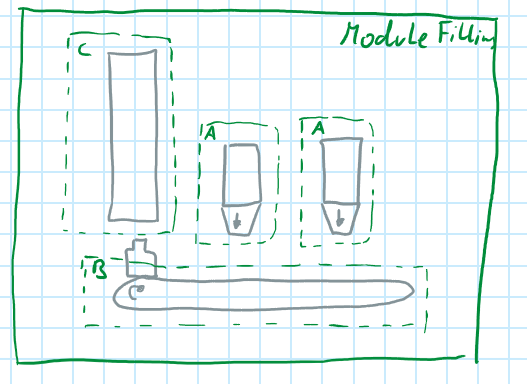
\includegraphics[width=.7\linewidth]{figures/StruktureCad.PNG}
		\caption{Layout of the filling station}
		\label{fig:DataStruktureUseLayout}
	\end{figure}

	The starting point for the development of the filling station are the exchange packages of the three suppliers with the respective product as content. These packages are connected and expanded and finally result in a package with the entire filling station as seen by the customer. In a next step, the customer is able to use the filling station in the planning of the remaining plant. This general procedure is shown in \autoref{fig:DataStruktureComponents}.
	\begin{figure}[htp]
		\centering
		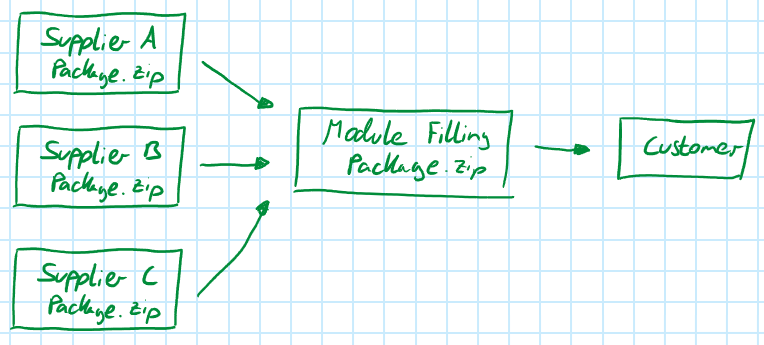
\includegraphics[width=.8\linewidth]{figures/StruktureFile.PNG}
		\caption{File components of the filling station}
		\label{fig:DataStruktureComponents}
	\end{figure}

	% Die tatsächliche Struktur
	The actual setup of the data structure is kept simple and consists of a root folder with several directories for the relevant information as shown in \autoref{fig:DataStruktureHierachry}. This root folder is finally compressed into a \textit{.zip} file for distribution. Due to the plain and simple structure, it can be easily extended and modularly exchanged.  
	\begin{figure}[htp]
		\centering
%		\footnotesize
		\scriptsize
		\tikzstyle{every node}=[draw=black,thick,anchor=west]
		\tikzstyle{basis}=[draw=black,fill=black!10]
		\begin{tikzpicture}[%
			grow via three points={one child at (0.5,-0.7) and
				two children at (0.5,-0.7) and (0.5,-1.4)},
			edge from parent path={(\tikzparentnode.south) |- (\tikzchildnode.west)}]
			\node [basis] {Data Structure}
			child { node {Geometry (CAD)}}		
			child { node {Control Software}}
			child { node {Behaviour Model}}
			child { node {Documentation}}
			child { node {\dots}}			
			child [missing] {}				
			child [missing] {}				
			child [missing] {};
		\end{tikzpicture}
		\caption{Data structure}
		\label{fig:DataStruktureHierachry}
	\end{figure}



\subsection{Used File Formats}
	As already mentioned in \autoref{sec:AvailableDataFormats}, a wide range of possible data formats exists to represent the required information for virtual commissioning. The focus in the selection of the used formats, should be on the widest possible support in different tools. Only through this approach the format can become accepted in the industry. In this section, the formats are selected and the result is summarized in \autoref{tab:InformationAndFormats}. \\

% Beschreibung und Begründung für alle Punkte
\subsubsection{Geometry and CAD}
	For a loss-free exchange of CAD data, the information of the kinematization of the assemblies must be preserved in addition to the raw geometry. As mentioned earlier, this is a big problem in practical use and therefore the \textit{COLLADA} format would be a optimal solution. At the moment, suitable tools for conversion are missing or do not support the current version of \textit{COLLADA} implementing the kinematization. As a result, using the \textit{COLLADA} format is the optimal solution in theory but in practice native CAD formats are the better choice. Which CAD tool and further which format is finally used has to be defined between the customer and supplier. Alternatively, neutral formats like \textit{.step} can be used, but with the disadvantage of missing kinematics. \\
	For example, \textit{Autodesk Inventor} offers a quick way to exchange data via the \textit{Pack and Go} tool \cite{InventorPackAndGo}. In this case, the entire geometry, dependencies and also materials of an assembly are bundled in one file, which also simplifies the exchange. A similar function is also available in \textit{Solidwork} \cite{SolidworksPackAndGo}. It should be noted, that although the two functions have the same name, they are not compatible with each other. \\

\subsubsection{Behaviour Model}
	The modeling of the physical behavior can also be done using various tools. In contrast to CAD data, a neutral and established format for data exchange already exists here: the \textit{FMI}. A growing number of tools support this format, making it a good choice in a modular virtual commissioning process. \\
	In the academic community, but also in industry, \textit{Matlab/Simulink} is often used for modelling. This tool is very popular mainly because of its flexibility, and supports the import and export of \textit{FMI} files in versions 1 and 2. Instructions for the export can be found in \cite{MatlabFmuExport} and for the import in \cite{MatlabFmuImport}. \\

% PLC Code
\subsubsection{PLC Code}
	The exchange of PLC code is almost no problem in practice. This is thanks to the standardization of automation engineering using PLCs, which also describes the possible programming languages and the exchange format as \textit{.xml} files. In addition to the language basis, more complex functions such as function blocks for movements are also part of the standard and thus easily exchangeable. Thanks to the international validity, many manufacturers rely on this standardization and offer converters to and from the \textit{PLCopen} format. \\

% Documentation and Drawings
\subsubsection{Documentation}
\colorbox{yellow}{To be added}


\begin{table}[htp]
	\scriptsize
	\centering
	\caption{Choosen file formats.}
	\begin{tabular}{ll}
		\toprule
		 \multicolumn{1}{c}{Information} & \multicolumn{1}{c}{Choosen File Format}\\
		 \midrule
		 CAD (pure geometry) & \textit{.step}\\
		 CAD (with kinematics) & Native or \textit{COLLADA}  \\
		 Pyhsical Behavior & \textit{FMU}\\
		 & \\
		 PLC Code & \textit{PLCopen} \\
		 & \\
		 Documentation & \textit{.pdf}\\
		 \bottomrule
	\end{tabular}	
	\label{tab:InformationAndFormats}
\end{table}



\section{Advantages and Disadvantages}
\colorbox{yellow}{To be added}


\section{Workflow of the proposed Data Structure}
% Introduction
\colorbox{yellow}{Description for \autoref{fig:GeneralWorkflow}}. 

\begin{figure}[htp]
	\centering
	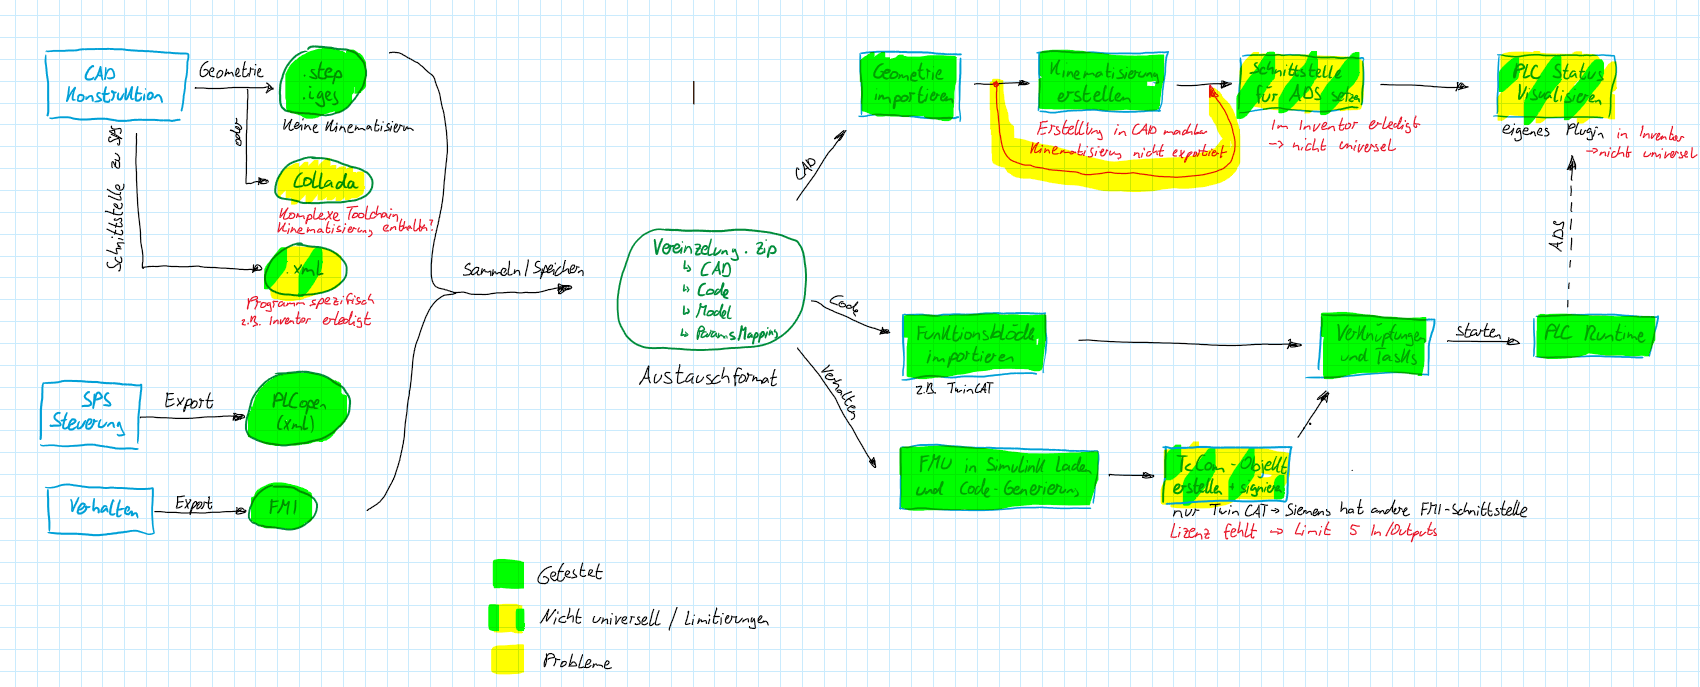
\includegraphics[width=.9\linewidth]{figures/GeneralWorkflow.PNG}
	\caption{General Workflow\colorbox{yellow}{bigger and maybe split into inport and export}}
	\label{fig:GeneralWorkflow}
\end{figure}




\section{Exemplary Application}
\colorbox{yellow}{to be added}
\begin{itemize}
	\item Introduction to used Hardware
	\item Workflow
	\item Finished Example
\end{itemize}

\section{Results and Conclusion}
\colorbox{yellow}{to be added}
\begin{itemize}
	\item Easier implementation 
	\item Depending on Software Inventor and TwinCAT
	\item CAD-Software is not open
\end{itemize}







% use section* for acknowledgement
\section*{Acknowledgment}


The authors would like to thank...

% references section

\bibliographystyle{IEEEtran}
\bibliography{IEEEexample}
% argument is your BibTeX string definitions and bibliography database(s)
%\bibliography{IEEEabrv,IEEEexample}


% biography section
%
% picture and CV only of main author

\begin{IEEEbiography}[{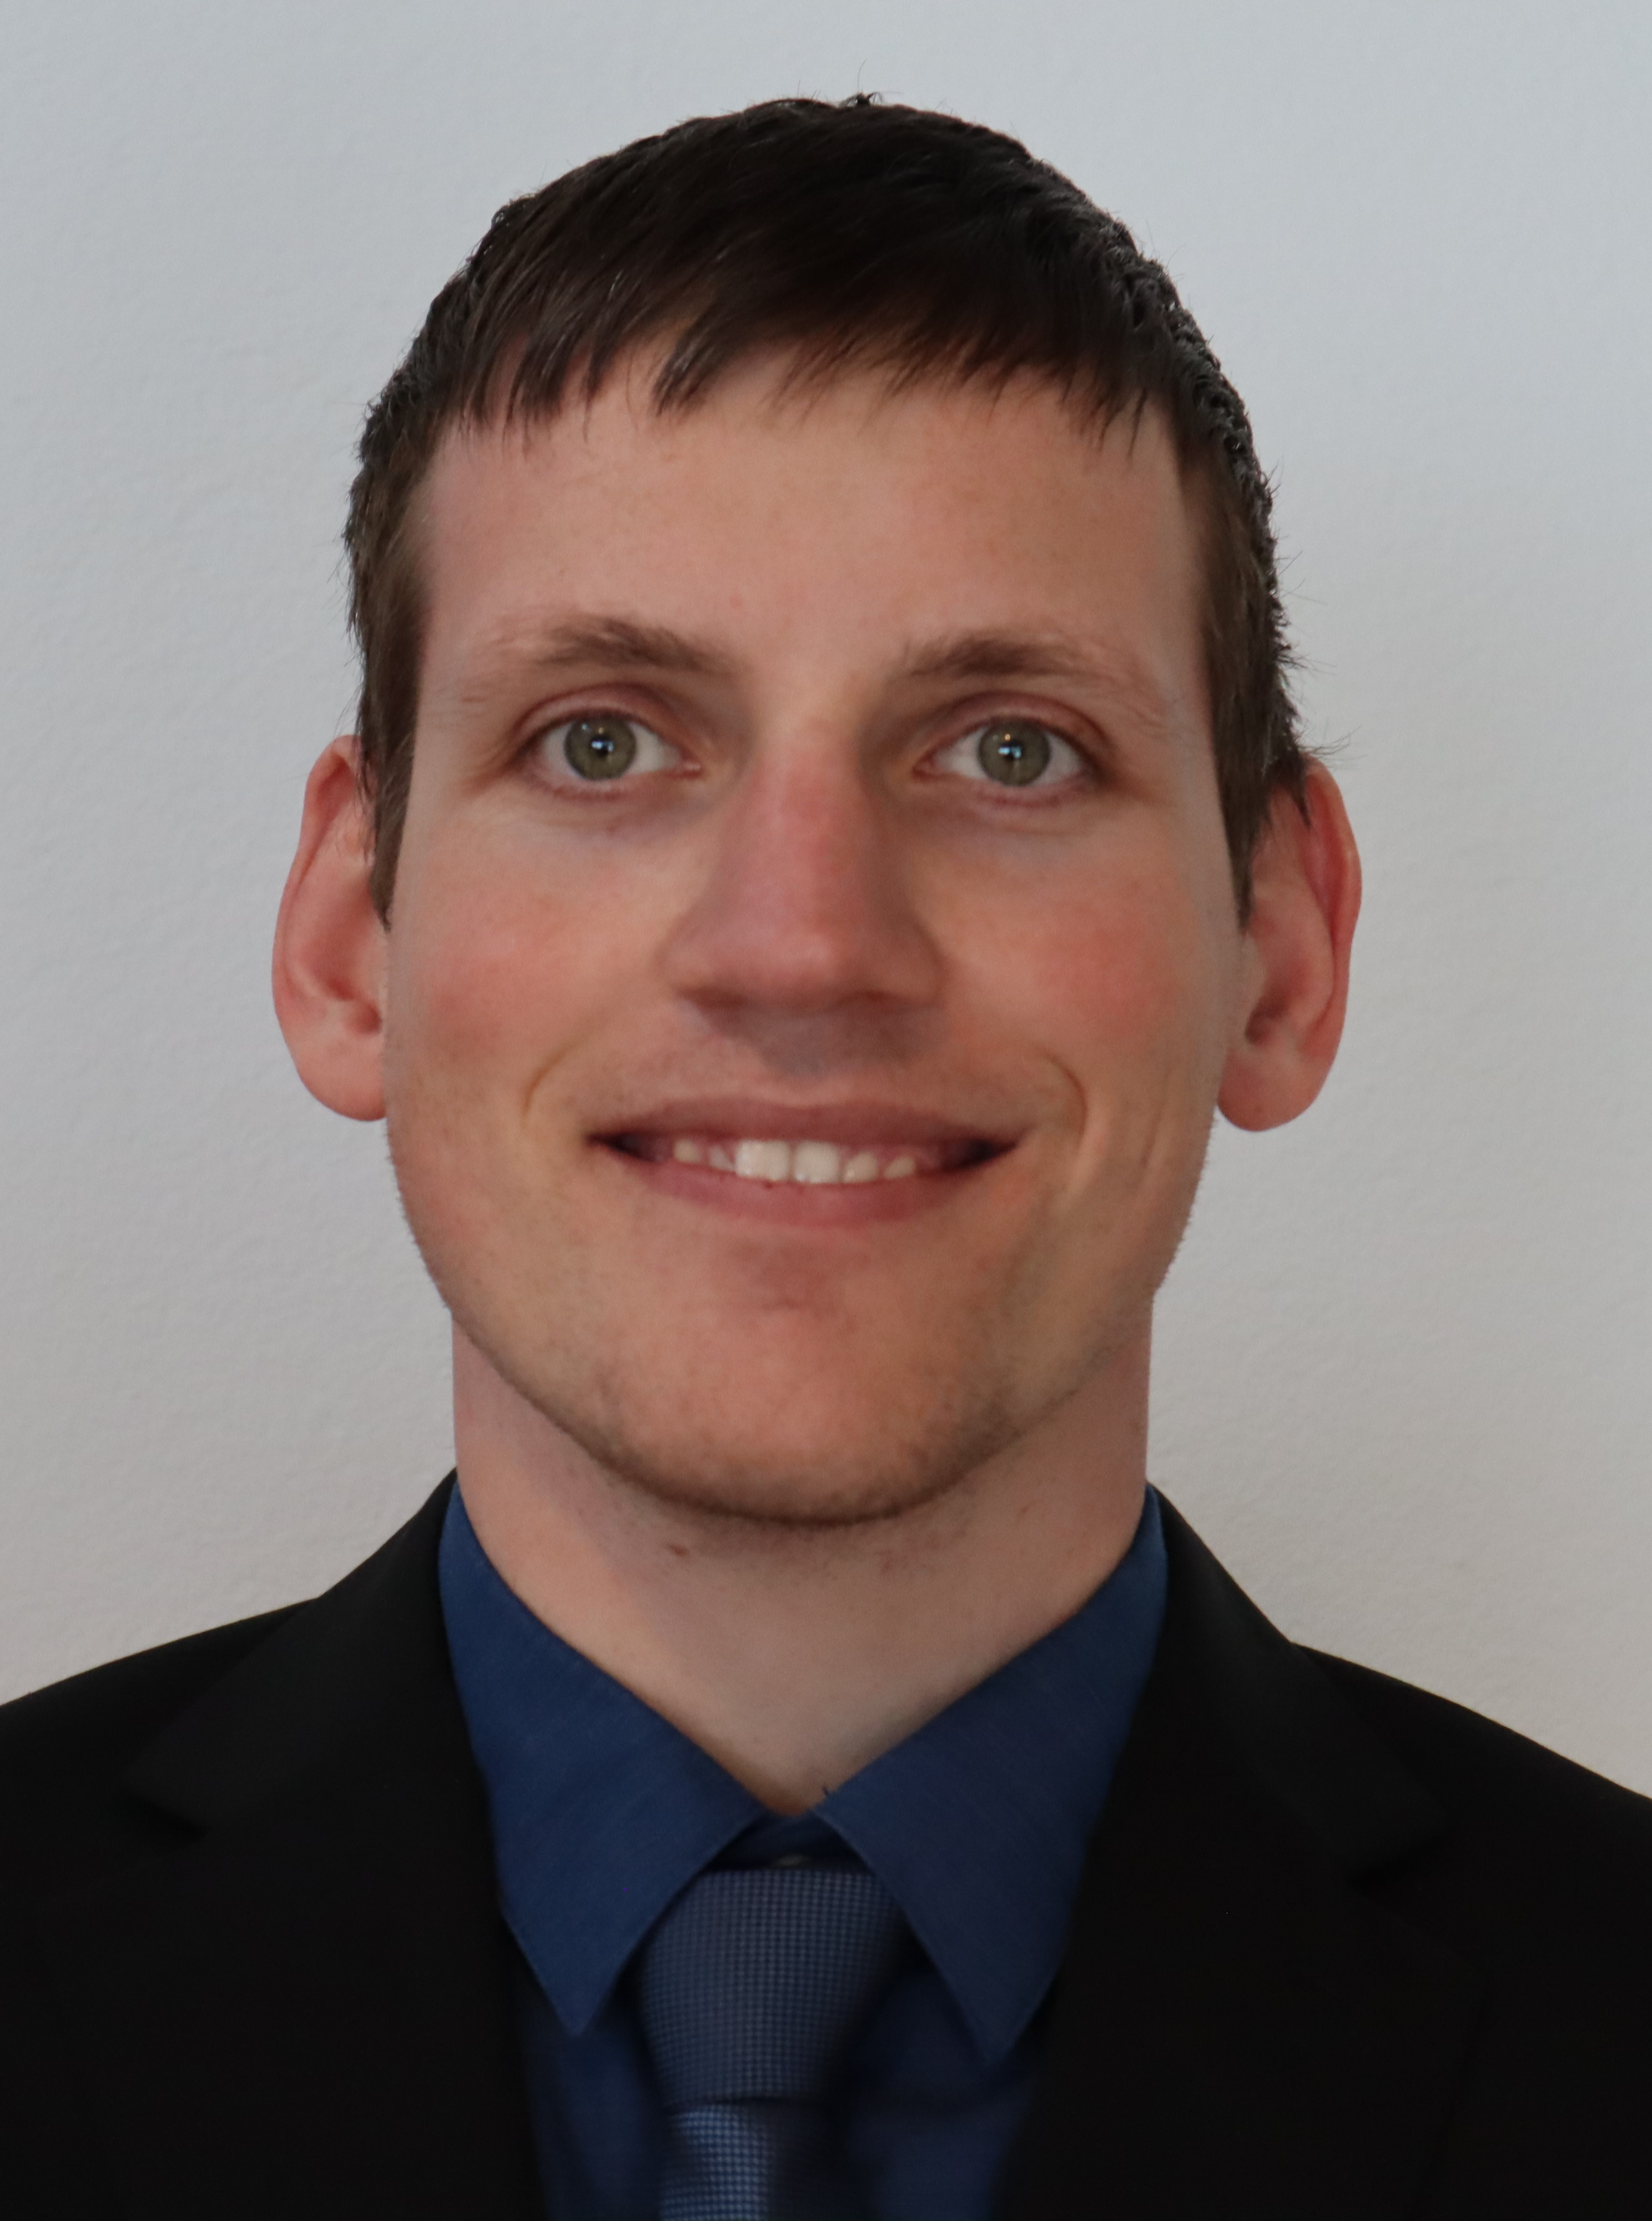
\includegraphics[width=1in,height=1.25in,clip,keepaspectratio]{DominiqueGeiger.JPG}}]{Dominique Geiger}
is Master student in the Department of Mechatronics at MCI Innsbruck/Austria.
\end{IEEEbiography}

% that's all folks
\end{document}

